\begin{frame}{Artificial Diamond Types}

	\begin{itemize}
		\item diamonds artificially grown with chemical vapour deposition (CVD)
		\item investigation of two different diamond types:
	\end{itemize}
	
	\begin{figure}[h] 
		\centering
		\begin{subfigure}{0.45\textwidth}  
			\centering
			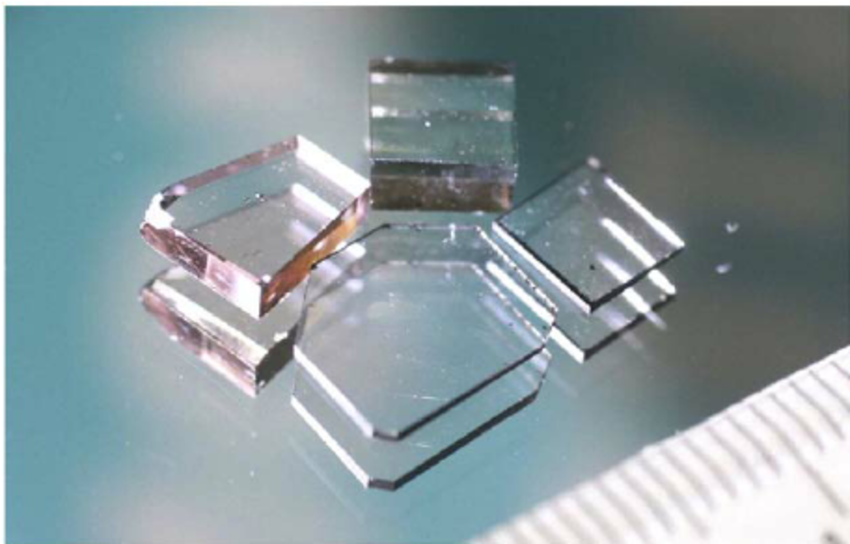
\includegraphics[height=0.4\textheight]{SCVD}
			\caption{single-crystalline CVD}
		\end{subfigure}
		\begin{subfigure}{0.45\textwidth} 
			\centering
			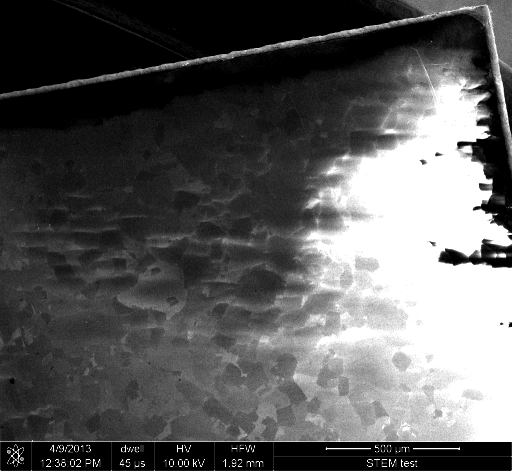
\includegraphics[height=0.4\textheight]{pCVD4}
			\caption{poly-crystalline CVD} 	
		\end{subfigure} 
	\end{figure}
	
	\begin{minipage}{5.5cm}
		\begin{itemize}
			\item grown on existing diamond crystal
			\item only small sizes (\SI{\sim.25}{cm^2})
			\item larger signals than pCVD ($5:3$)
		\end{itemize}
	\end{minipage}
	\hspace*{.5cm}
	\begin{minipage}{5cm}
		\begin{itemize}
			\item grown on Si substrate with diamond powder
			\item large wafers (\SIrange{5}{6}{''} \diameter)
			\item non-uniformities and grains
		\end{itemize}
	\end{minipage}
	
\end{frame}
